% Ejemplo dorado de slides -- reconstruido a partir de dos presentaciones
% reales del profesor ("Ecuación de energía en tuberías.key" y
% "Coeficiente de Coriolis para tuberías.key", Hidráulica Aplicada),
% fusionadas y corregidas en sesión de diseño. Cambios de fondo respecto
% al original (no solo de estilo):
%   1. La razón de calor se llamaba "H" -- choca con la notación estándar
%      de entalpía. Se usa Q_H (Streeter) en vez de Q a secas, porque Q
%      ya está reservado para caudal en todo el curso -- decisión
%      explícita del profesor, no una convención inventada por el agente.
%   2. El coeficiente de corrección de energía (alpha) se introducía 3
%      diapositivas después del paso exacto donde hace falta
%      (∫ρv³dA = ρV³A solo es cierto en flujo uniforme) -- ahora se
%      define en ese mismo paso y se arrastra hasta la ecuación final.
%   3. La diapositiva 3 de "Coeficiente de Coriolis" tenía (γ/2g)v³/dA
%      con dA dividiendo -- error algebraico/dimensional, corregido a
%      (γ/2g)v³dA (dA multiplicando), consistente con la integral de la
%      diapositiva siguiente.
%   4. La explicación del signo del trabajo de flujo en la entrada era
%      confusa ("la fuerza actúa en dirección opuesta al movimiento de
%      la frontera") -- reescrita como el argumento estándar: el entorno
%      empuja al sistema en la entrada (trabajo negativo hecho por el
%      sistema), el sistema empuja al entorno en la salida (trabajo
%      positivo).
% Los tres diagramas (volumen de control, perfil de velocidad, línea de
% gradiente de energía) son versiones simplificadas propias en TikZ, no
% reproducciones de las figuras originales del profesor.
\DocumentMetadata{lang=es-DO,tagging=on,pdfstandard=ua-2}
\documentclass{ltx-talk}
\usepackage{icv}
\usepackage{tikz}

\DeclareColor{structure}[HTML]{005DAA}

% -----------------------------------------------------------------------
% Metadata
% -----------------------------------------------------------------------
\icvsetup{
  asignatura  = {ICV 441-T -- Hidráulica Aplicada},
  titulocorto = {Ecuación de energía en tuberías},
  titulo      = {Ecuación de Energía en Tuberías},
  subtitulo   = {Del Teorema de Transporte de Reynolds al coeficiente de Coriolis},
  profesor    = {Dr. Ricardo Hernández Moreira},
  periodo     = \icvciclo{2026}{3},
  version     = {v1},
}

\makeatletter
\title{\icv@titulo}
\subtitle{\icv@subtitulo}
\author{\icv@profesor}
\institute{\icv@asignatura}
\date{\icv@periodo}
\makeatother

\EditInstance{footer}{std}{
  background-color = icvblue,
  color            = white,
  element-order    = {institute, title, framenumber},
}

\begin{document}

\begin{frame}
  \maketitle[framestyle = wallpaper, horizontal-alignment = left]
\end{frame}

\begin{frame}
  \frametitle{Objetivos de aprendizaje}
  \begin{icvobjectives}
    \item Derivar la ecuación general de energía para un volumen de
      control a partir de la Primera Ley de la Termodinámica y el
      Teorema de Transporte de Reynolds.
    \item Interpretar cada término de la ecuación de energía en
      tuberías como una altura (de presión, cinética, de elevación,
      de pérdida).
    \item Definir y calcular el coeficiente de corrección de energía
      $\alpha$ (Coriolis) para un perfil de velocidad no uniforme.
  \end{icvobjectives}
\end{frame}

\begin{frame}
  \frametitle{Primera ley de la termodinámica}
  La razón de cambio en el tiempo de la energía $E$ de un sistema es
  igual a la razón de transferencia de calor hacia el fluido menos la
  razón a la que el fluido realiza trabajo sobre su entorno:
  \[
    \frac{dE}{dt} = \frac{dQ_H}{dt} - \frac{dW}{dt}
  \]

  \vspace{0.5em}
  \begin{icvnote}[Notación]
  Se usa $Q_H$ para la razón de calor (siguiendo a Streeter) en vez de
  $Q$ a secas: en este curso $Q$ ya está reservado para caudal, y usarlo
  también para calor generaría confusión constante.
  \end{icvnote}
\end{frame}

\begin{frame}
  \frametitle{Energía total en un fluido}
  La energía total en el fluido es la suma de la energía interna $E_u$,
  cinética $E_k$ y potencial $E_p$:
  \[
    E = E_u + E_k + E_p
  \]
\end{frame}

\begin{frame}
  \frametitle{Propiedades extensiva e intensiva del sistema}
  La propiedad extensiva del Teorema de Transporte de Reynolds (TTR) es
  la energía, $B = E$:
  \[
    B = E_u + E_k + E_p
  \]
  La propiedad intensiva correspondiente es la energía por unidad de
  masa, $\beta$:
  \[
    \beta = \frac{dB}{dm} = e_u + e_k + e_p
  \]
  donde los subíndices $u$, $k$ y $p$ denotan energía por unidad de masa
  interna, cinética y potencial, respectivamente.
\end{frame}

\begin{frame}
  \frametitle{Ecuación de balance de energía}
  Aplicando el TTR a la propiedad extensiva $B = E$:
  \begin{align*}
    \frac{dB}{dt} = \frac{dE}{dt} &= \frac{dQ_H}{dt} - \frac{dW}{dt} \\
      &= \frac{d}{dt}\int_{CV} (e_u+e_k+e_p)\,\rho\,d\forall
         \;+\; \sum_{CS} (e_u+e_k+e_p)\,\rho\,\mathbf{V}\cdot\mathbf{A}
  \end{align*}
\end{frame}

\begin{frame}
  \frametitle{Energía cinética y potencial por unidad de masa}
  \[
    e_k = \frac{mV^2/2}{m} = \frac{V^2}{2}
  \]
  \vspace{1em}
  \[
    e_p = \frac{\gamma \forall z}{m} = \frac{\gamma \forall z}{\rho \forall} = gz
  \]
  \vspace{0.5em}

  donde $\forall$ denota volumen y $\gamma = \rho g$ es el peso
  específico.
\end{frame}

\begin{frame}
  \frametitle{Ecuación general de energía}
  \framesubtitle{Flujo no permanente, variado, de densidad variable}
  \[
    \frac{dQ_H}{dt} - \frac{dW}{dt}
      = \frac{d}{dt}\int_{CV}\Bigl(e_u+\tfrac{1}{2}V^2+gz\Bigr)\rho\,d\forall
        + \sum_{CS}\Bigl(e_u+\tfrac{1}{2}V^2+gz\Bigr)\rho\,\mathbf{V}\cdot\mathbf{A}
  \]
\end{frame}

\begin{frame}
  \frametitle{Ecuación de energía}
  \framesubtitle{Flujo permanente, variado, de densidad variable}
  Para flujo permanente se anula el término de acumulación en el
  volumen de control:
  \[
    \frac{dQ_H}{dt} - \frac{dW}{dt}
      = \sum_{CS}\Bigl(e_u+\tfrac{1}{2}V^2+gz\Bigr)\rho\,\mathbf{V}\cdot\mathbf{A}
  \]
\end{frame}

\begin{frame}
  \frametitle{Consideraciones sobre el trabajo $W$}
  \begin{itemize}
    \item El trabajo realizado por el sistema puede dividirse en:
    \begin{enumerate}
      \item Trabajo de eje o trabajo en la flecha, $W_s$.
      \item Trabajo de flujo, $W_f$.
    \end{enumerate}
    \item El trabajo de flujo es el resultado de la fuerza producida
      por la presión a medida que el sistema se mueve por el espacio.
    \item El trabajo de eje es cualquier otro trabajo que no sea
      trabajo de flujo (p.\,ej.\ el que entrega o recibe una turbomáquina).
  \end{itemize}
\end{frame}

\begin{frame}
  \frametitle{Recordemos el volumen de control}
  \begin{center}
  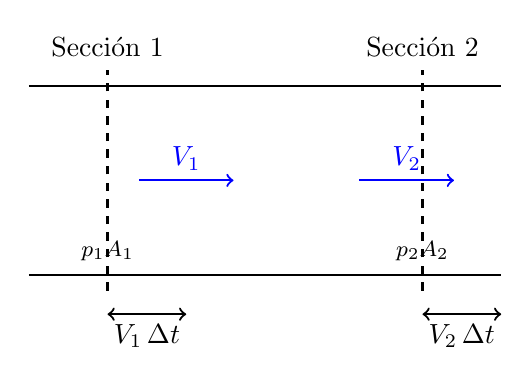
\begin{tikzpicture}[x=1cm,y=1cm,thick]
    % Duct walls
    \draw (0,1.2) -- (6,1.2);
    \draw (0,-1.2) -- (6,-1.2);
    % Sections 1 and 2
    \draw[dashed] (1,-1.4) -- (1,1.4);
    \draw[dashed] (5,-1.4) -- (5,1.4);
    \node at (1,1.7) {Sección 1};
    \node at (5,1.7) {Sección 2};
    % Flow direction
    \draw[->, blue] (1.4,0) -- (2.6,0) node[midway,above]{$V_1$};
    \draw[->, blue] (4.2,0) -- (5.4,0) node[midway,above]{$V_2$};
    % Distance traveled markers
    \draw[<->] (1,-1.7) -- (2,-1.7) node[midway,below]{$V_1\,\Delta t$};
    \draw[<->] (5,-1.7) -- (6,-1.7) node[midway,below]{$V_2\,\Delta t$};
    % Force labels
    \node at (1,-0.9) {\footnotesize $p_1 A_1$};
    \node at (5,-0.9) {\footnotesize $p_2 A_2$};
  \end{tikzpicture}
  \end{center}
  En el volumen de control, la fuerza $F_1$ en el lado aguas arriba del
  fluido es $p_1 A_1$; en el lado aguas abajo es $F_2 = p_2 A_2$. La
  frontera del sistema en cada sección se desplaza la distancia
  recorrida en el tiempo $\Delta t$: $l_1 = V_1\Delta t$,
  $l_2 = V_2\Delta t$.
\end{frame}

\begin{frame}
  \frametitle{Trabajo de flujo: signo}
  El trabajo realizado por cada fuerza de presión es el producto de la
  fuerza por la distancia recorrida:
  \begin{itemize}
    \item En la \textbf{entrada}, el entorno (aguas arriba) empuja al
      sistema -- hace trabajo \emph{sobre} el sistema, que es trabajo
      \emph{negativo} hecho \emph{por} el sistema:
      \[
        W_{f_1} = -V_1\,p_1\,A_1\,\Delta t
      \]
    \item En la \textbf{salida}, el sistema empuja al entorno (aguas
      abajo) -- trabajo \emph{positivo} hecho por el sistema:
      \[
        W_{f_2} = V_2\,p_2\,A_2\,\Delta t
      \]
  \end{itemize}
\end{frame}

\begin{frame}
  \frametitle{Razón de trabajo de flujo en el tiempo}
  \begin{align*}
    \text{Aguas arriba:} \quad & \frac{dW_{f_1}}{dt} = -V_1\,p_1\,A_1 \\[0.5em]
    \text{Aguas abajo:} \quad & \frac{dW_{f_2}}{dt} = V_2\,p_2\,A_2 \\[0.5em]
    \text{En general, para todas las corrientes:} \quad
      & \frac{dW_f}{dt} = \sum_{CS} p\,\mathbf{V}\cdot\mathbf{A}
        = \sum_{CS} \frac{p}{\rho}\,\rho\,\mathbf{V}\cdot\mathbf{A}
  \end{align*}
\end{frame}

\begin{frame}
  \frametitle{Razón neta de trabajo sobre el sistema}
  \[
    \frac{dW}{dt} = \frac{dW_s}{dt} + \sum_{CS} \frac{p}{\rho}\,\rho\,\mathbf{V}\cdot\mathbf{A}
  \]
\end{frame}

\begin{frame}
  \frametitle{Ecuación general de energía}
  \framesubtitle{Sustituyendo $W = W_s + W_f$}
  \begin{align*}
    \frac{dQ_H}{dt} - \frac{dW_s}{dt} - \sum_{CS}\frac{p}{\rho}\rho\mathbf{V}\cdot\mathbf{A}
      &= \frac{d}{dt}\int_{CV}\Bigl(e_u+\tfrac{1}{2}V^2+gz\Bigr)\rho\,d\forall
         + \sum_{CS}\Bigl(e_u+\tfrac{1}{2}V^2+gz\Bigr)\rho\mathbf{V}\cdot\mathbf{A}
  \end{align*}
  que se simplifica a:
  \[
    \frac{dQ_H}{dt} - \frac{dW_s}{dt}
      = \frac{d}{dt}\int_{CV}\Bigl(e_u+\tfrac{V^2}{2}+gz\Bigr)\rho\,d\forall
        + \sum_{CS}\Bigl(\frac{p}{\rho}+e_u+\tfrac{V^2}{2}+gz\Bigr)\rho\mathbf{V}\cdot\mathbf{A}
  \]
\end{frame}

\begin{frame}
  \frametitle{Ecuación de energía}
  \framesubtitle{Flujo permanente}
  \[
    \frac{dQ_H}{dt} - \frac{dW_s}{dt}
      = \sum_{CS}\Bigl(\frac{p}{\rho}+e_u+\tfrac{V^2}{2}+gz\Bigr)\rho\mathbf{V}\cdot\mathbf{A}
  \]
  De forma más general, como integral sobre la superficie de control:
  \[
    \frac{dQ_H}{dt} - \frac{dW_s}{dt}
      = \int_{CS}\Bigl(\frac{p}{\rho}+e_u+\tfrac{V^2}{2}+gz\Bigr)\rho\,\mathbf{V}\cdot d\mathbf{A}
  \]
\end{frame}

\begin{frame}
  \frametitle{Flujo en tubería: entrada y salida}
  \begin{center}
  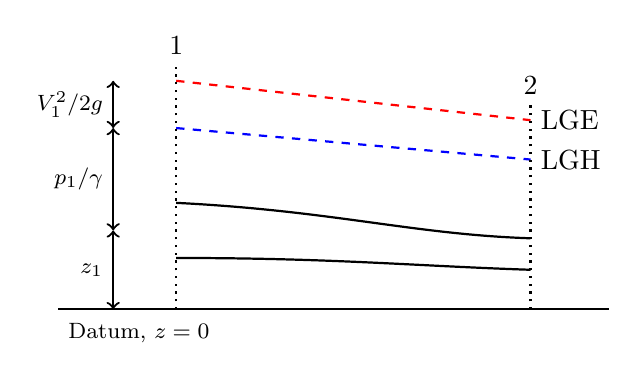
\begin{tikzpicture}[x=1cm,y=1cm,thick]
    \draw (0,0) -- (7,0); % datum
    \node[anchor=north west] at (0,-0.05) {\footnotesize Datum, $z=0$};
    % pipe (converging duct)
    \draw (1.5,1.35) .. controls (3.5,1.25) and (4.5,0.95) .. (6,0.9);
    \draw (1.5,0.65) .. controls (3.5,0.65) and (4.5,0.55) .. (6,0.5);
    % EGL and HGL
    \draw[dashed,red]  (1.5,2.9) -- (6,2.4) node[right,black]{LGE};
    \draw[dashed,blue] (1.5,2.3) -- (6,1.9) node[right,black]{LGH};
    % section markers
    \draw[dotted] (1.5,0) -- (1.5,3.1);
    \draw[dotted] (6,0) -- (6,2.6);
    \node[above] at (1.5,3.1) {1};
    \node[above] at (6,2.6) {2};
    % height brackets at section 1, offset left of the section line
    \draw[<->] (0.7,0)   -- (0.7,1.0) node[midway,left]{\footnotesize $z_1$};
    \draw[<->] (0.7,1.0) -- (0.7,2.3) node[midway,left]{\footnotesize $p_1/\gamma$};
    \draw[<->] (0.7,2.3) -- (0.7,2.9) node[midway,left]{\footnotesize $V_1^2/2g$};
  \end{tikzpicture}
  \end{center}
  Suponiendo flujo en una tubería, definimos secciones en la entrada
  (1) y la salida (2). LGE = línea de gradiente de energía, LGH = línea
  de gradiente hidráulica.
\end{frame}

\begin{frame}
  \frametitle{Reducción a las secciones 1 y 2}
  \begin{align*}
    \frac{dQ_H}{dt} - \frac{dW_s}{dt}
      &= \int_{A_2}\Bigl(\frac{p_2}{\rho}+e_{u_2}+\tfrac{V_2^2}{2}+gz_2\Bigr)\rho V_2\,dA_2 \\
      &\quad - \int_{A_1}\Bigl(\frac{p_1}{\rho}+e_{u_1}+\tfrac{V_1^2}{2}+gz_1\Bigr)\rho V_1\,dA_1
  \end{align*}
  Separando el término cinético ($\tfrac{1}{2}V^2\rho V\,dA = \tfrac{1}{2}\rho V^3\,dA$):
  \begin{align*}
    \frac{dQ_H}{dt} - \frac{dW_s}{dt}
      &= \int_{A_2}\Bigl(\frac{p_2}{\rho}+e_{u_2}+gz_2\Bigr)\rho V_2\,dA_2
         + \int_{A_2} \frac{\rho V_2^3}{2}\,dA_2 \\
      &\quad - \int_{A_1}\Bigl(\frac{p_1}{\rho}+e_{u_1}+gz_1\Bigr)\rho V_1\,dA_1
         - \int_{A_1} \frac{\rho V_1^3}{2}\,dA_1
  \end{align*}
\end{frame}

\begin{frame}
  \frametitle{Condición hidrostática y coeficiente $\alpha$}
  El flujo es uniforme (unidireccional) en las secciones 1 y 2, así que
  prevalecen condiciones hidrostáticas -- $p/\rho + e_u + gz$ es
  constante en cada sección, y sale de la integral:
  \[
    \int_A \Bigl(\frac{p}{\rho}+e_u+gz\Bigr)\rho V\,dA
      = \Bigl(\frac{p}{\rho}+e_u+gz\Bigr)\dot{m}
  \]

  El término cinético \textbf{no} sale así de fácil: $\int_A \rho V^3\,dA
  = \rho \bar{V}^3 A$ solo si el perfil de velocidad es uniforme. Para
  un perfil real, se define el \textbf{coeficiente de corrección de
  energía} $\alpha$ precisamente aquí:
  \[
    \int_A \frac{\rho V^3}{2}\,dA = \alpha\,\dot{m}\,\frac{\bar{V}^2}{2},
    \qquad
    \alpha \equiv \frac{1}{A\bar{V}^3}\int_A V^3\,dA
  \]
\end{frame}

\begin{frame}
  \frametitle{Sustituyendo el flujo másico}
  Con $\dot{m} = \int_A \rho V\,dA$ y $\alpha$ ya incorporado:
  \[
    \frac{dQ_H}{dt} - \frac{dW_s}{dt}
      = \Bigl(\frac{p_2}{\rho}+e_{u_2}+gz_2\Bigr)\dot m + \alpha_2\,\dot m\,\frac{V_2^2}{2}
        - \Bigl(\frac{p_1}{\rho}+e_{u_1}+gz_1\Bigr)\dot m - \alpha_1\,\dot m\,\frac{V_1^2}{2}
  \]
  Dividiendo entre el flujo de masa y reorganizando:
  \[
    \frac{1}{\dot m}\Bigl(\frac{dQ_H}{dt}-\frac{dW_s}{dt}\Bigr)
      + \frac{p_1}{\rho}+e_{u_1}+gz_1+\alpha_1\frac{V_1^2}{2}
      = \frac{p_2}{\rho}+e_{u_2}+gz_2+\alpha_2\frac{V_2^2}{2}
  \]
\end{frame}

\begin{frame}
  \frametitle{Trabajo de eje: bombas y turbinas}
  El trabajo de eje se descompone en lo que entrega una turbina y lo
  que consume una bomba:
  \[
    \frac{dW_s}{dt} = \frac{dW_T}{dt} - \frac{dW_P}{dt}
  \]
  Sustituyendo, dividiendo entre la gravedad y reorganizando:
  \begin{align*}
    \frac{1}{\dot m g}\frac{dW_P}{dt} + \frac{p_1}{\rho g}+z_1+\alpha_1\frac{V_1^2}{2g}
      &= \frac{1}{\dot m g}\frac{dW_T}{dt} + \frac{p_2}{\rho g}+z_2+\alpha_2\frac{V_2^2}{2g} \\
      &\quad + \left[\frac{e_{u_2}-e_{u_1}}{g} - \frac{1}{\dot m g}\frac{dQ_H}{dt}\right]
  \end{align*}
\end{frame}

\begin{frame}
  \frametitle{Definiendo las alturas}
  \[
    h_P = \frac{1}{\dot m g}\frac{dW_P}{dt}
    \qquad
    h_T = \frac{1}{\dot m g}\frac{dW_T}{dt}
  \]
  \[
    h_L = \left(\frac{e_{u_2}-e_{u_1}}{g}\right) - \frac{1}{\dot m g}\frac{dQ_H}{dt}
  \]
  $h_P$ y $h_T$ son la altura suplida por bombas y turbinas; $h_L$ es
  la pérdida de altura -- energía mecánica convertida irreversiblemente
  en energía interna (calor) por esfuerzos viscosos.
\end{frame}

\begin{frame}
  \frametitle{Ecuación de energía}
  Sustituyendo, y usando $\gamma = \rho g$:
  \begin{icvwarning}[Resultado clave]
  \[
    \frac{p_1}{\gamma}+z_1+\alpha_1\frac{V_1^2}{2g}+h_P
      = \frac{p_2}{\gamma}+z_2+\alpha_2\frac{V_2^2}{2g}+h_T+h_L
  \]
  \end{icvwarning}
  \vspace{0.5em}
  \begin{itemize}
    \item $p/\gamma$ es la altura de presión; $p/\gamma + z$, la altura
      piezométrica; $\alpha V^2/2g$, la altura cinética corregida.
    \item Esta ecuación supone que $V$ es la velocidad promedio en la
      sección -- por eso hace falta $\alpha$.
  \end{itemize}
\end{frame}

\begin{frame}
  \frametitle{¿De dónde sale exactamente $\alpha$?}
  \framesubtitle{Una derivación alternativa, más intuitiva}
  \begin{center}
  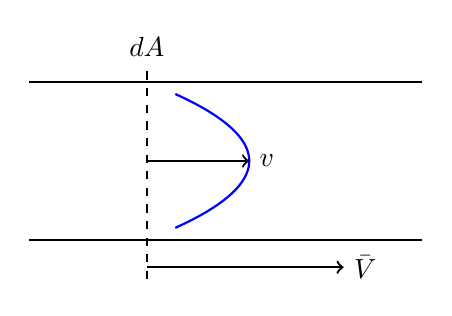
\begin{tikzpicture}[x=1cm,y=1cm,thick]
    \draw (0,1) -- (5,1);
    \draw (0,-1) -- (5,-1);
    \draw[domain=-0.85:0.85,smooth,variable=\y,blue]
      plot ({1.3*(1-\y*\y)+1.5},{\y});
    \draw[->] (1.5,0) -- (2.8,0) node[right]{$v$};
    \draw[->] (1.5,-1.35) -- (4,-1.35) node[right]{$\bar V$};
    \draw[dashed] (1.5,-1.5) -- (1.5,1.2);
    \node[above] at (1.5,1.2) {$dA$};
  \end{tikzpicture}
  \end{center}
  El perfil de velocidad real $v$ varía en la sección transversal, y no
  es igual a la velocidad promedio $\bar V$ en todos los puntos.
\end{frame}

\begin{frame}
  \frametitle{Flujo real de energía cinética}
  La masa de fluido que atraviesa un área $dA$ por unidad de tiempo es
  $(\gamma/g)\,v\,dA$. El flujo de energía cinética a través de esa
  misma área es:
  \[
    (\gamma/g)\,v\,dA\left(\frac{v^2}{2}\right) = \frac{\gamma}{2g}\,v^3\,dA
  \]
  Integrando sobre toda la sección, la energía cinética total real que
  fluye por unidad de tiempo es:
  \[
    \dot{E}_{k,\text{real}} = \frac{\gamma}{2g}\int_A v^3\,dA
  \]
\end{frame}

\begin{frame}
  \frametitle{Flujo idealizado con velocidad promedio}
  Usando la velocidad promedio $\bar V$ junto con el coeficiente
  $\alpha$, la energía cinética por unidad de masa es
  $\alpha \bar V^2/2g$; el caudal a través de la sección es
  $\gamma A \bar V$. La energía cinética total \emph{idealizada} es
  entonces:
  \[
    \dot{E}_{k,\text{ideal}} = \gamma A \bar V \left(\alpha\,\frac{\bar V^2}{2g}\right)
      = \alpha\,\gamma A\,\frac{\bar V^3}{2g}
  \]
\end{frame}

\begin{frame}
  \frametitle{Resolviendo para $\alpha$}
  Igualando el flujo real (dos diapositivas atrás) con el flujo
  idealizado y resolviendo para $\alpha$:
  \[
    \frac{\gamma}{2g}\int_A v^3\,dA = \alpha\,\gamma A\,\frac{\bar V^3}{2g}
  \]
  \begin{icvwarning}[Resultado clave]
  \[
    \alpha = \frac{1}{A\bar V^3}\int_A v^3\,dA
  \]
  \end{icvwarning}
  Exactamente la misma definición a la que llegamos antes, por un
  camino distinto -- comparando la energía cinética real contra la que
  tendríamos si toda la sección se moviera a la velocidad promedio.
\end{frame}

\begin{frame}
  \frametitle{Valores típicos de $\alpha$}
  \begin{center}
  \begin{tabular}{ll}
    \toprule
    \textbf{Perfil de velocidad} & \textbf{$\alpha$ típico} \\
    \midrule
    Uniforme (flujo tapón) & $1.0$ \\
    Turbulento (tubería) & $1.03$--$1.06$ \\
    Laminar (tubería) & $2.0$ \\
    \bottomrule
  \end{tabular}
  \end{center}
  \vspace{0.5em}
  En la práctica de ingeniería, $\alpha \approx 1$ es una aproximación
  razonable para flujo turbulento -- el caso más común en sistemas de
  agua potable y alcantarillado.
\end{frame}

\end{document}
